\documentclass{article} % For LaTeX2e
\usepackage{final_project,times}
%\documentstyle[nips12submit_09,times,art10]{article} % For LaTeX 2.09
\usepackage{amsmath,amsthm,amsfonts,amssymb,amscd}
\usepackage{fullpage}
\usepackage{lastpage}
\usepackage{enumerate}
\usepackage{fancyhdr}
\usepackage{mathrsfs}
\usepackage{xcolor}
\usepackage[margin=2cm]{geometry}
\usepackage{fancyhdr} % Required for custom headers
\usepackage{lastpage} % Required to determine the last page for the footer
\usepackage{extramarks} % Required for headers and footers
\usepackage{graphicx} % Required to insert images
\usepackage{listings} % Required for insertion of code
\usepackage{framed}
\usepackage{courier}  % Required for the courier font
\usepackage{lipsum} % Used for inserting dummy 'Lorem ipsum' text into the template
\usepackage{float}
\usepackage{url}
\usepackage{bbm}
\usepackage{relsize}
\usepackage{amssymb}
\usepackage{fancyvrb}
\usepackage{amsmath}
\usepackage{mathrsfs}
\usepackage{algorithm}
\usepackage[noend]{algpseudocode}
\usepackage{amsmath}
\usepackage{listings}
\usepackage[none]{hyphenat}

\title{Optimizing Preseason Fantasy Football Rankings}

\author{
John O'Hollaren (jpo4) \\
Department of Electrical and Computer Engineering\\
}

\newcommand{\fix}{\marginpar{FIX}}
\newcommand{\new}{\marginpar{NEW}}

\nipsfinalcopy

\begin{document}


\maketitle

%#####################################################################################
%	Abstract
%#####################################################################################

\begin{abstract}
Fantasy football is a fast growing, multi-billion dollar industry centered around projecting which players will perform the best over the course of a season. Correctly predicting which players will play well greatly improves your team's year-long performance, whereas wasting a high pick on a low achiever can ruin your season. This paper focuses on an optimal strategy for predicting which NFL wide receivers will have the best fantasy football season using data available prior to the beginning of the season.
\end{abstract}

%#####################################################################################
%	Introduction & Related Work
%#####################################################################################

\section{Introduction \& Related Work}

According to the Fantasy Sports Trade Association, over 10 percent of the US population spent 12 billion dollars playing fantasy football in 2012. Given such a large market, a slight statistical advantage could provide significant profits in fantasy football leagues. Specifically, a correct pre-season ranking of wide receivers (WRs) will allow owners to pick the best players to join their teams during the pre season fantasy football draft, setting them up for year-long success. However, ranking players is difficult. Preseason rankings from teams of experts at ESPN and Yahoo are correct for only a small minority of players. This paper compares several machine learning techniques for ranking WRs, including linear regression, feature reduction, k-means clustering, mixture models, and PCA. A PCA regression technique which outperforms ESPN and Yahoo experts is presented.

While countless fantasy football websites exist, the major players are ESPN, Yahoo, the NFL, 4for4, and FantasyPros. None of these entities releases their methods publicly. Tim Mathews at the University of Southampton\footnote{Mathews, Tim, et. al. �Competing with Humans at Fantasy Football: Team Formation in Large Partially-Observable Domain.� Association for the Advancement of Artificial Intelligence, 2012.} explored using Bayesian reinforcement learning for week-to-week team management during the season. Matt Bookman at Stanford used linear regression to predict week-to-week performances during the season with limited success only in certain weeks\footnote{Bookman, Matt. "Predicting Fantasy Football - Truth in Data." Stanford CS 229 Final Project. December 14, 2012.}. The week-to-week prediction problem, however, is simplified through the use in-season data from each player, whereas in the pre-season, year-long ranking problem, predictions must be made for players who are 8 months removed from public games. Some attempts at machine learning approaches for the year-long ranking problem have been made\footnote{Kapania, Nitin. "Predicting Fantasy Football Performance with Machine Learning Techniques." Stanford CS 229 Final Project. December 14, 2012}, but did not outperform human experts. Other attempts use machine learning to outsmart other players in the same league\footnote{Becker, Adrian, et. al. "An Analytical Approach for Fantasy Football Draft and Lineup Management." MIT ORC Technical Report. November 2010.}. 

\subsection{How Does Fantasy Football Work?}

Points are awarded when a player scores a touchdown or gains yards. Each owner picks their team at the beginning of the year. Correctly predicting which players will play well greatly improves your team's year-long performance. This paper focuses on an optimal strategy for predicting a list of the top 30 non-rookie NFL wide receivers for a season, using only data available prior to the start of the season..

\subsection{Data Summarization}

My dataset includes NFL statistics for over 700 players for every year from 2007 to 2012. There are 13 features in total: Receiving Yards, Receiving Touchdowns, Receiving Targets, Receiving Catches, ESPN Preseason Ranking, Yahoo Preseason Ranking, $\Delta$1 year Receiving Yards: (Yards in year Y-1) - (Yards in year Y-2), $\Delta$1 year Receiving TDs: (TDs in year Y-1) - (TDs in year Y-2), $\Delta$2 year Receiving Yards: (Yards in year Y-1)-(Yards in year Y-3), $\Delta$2 year Receiving TDs: (TDs in year Y-1) - (TDs in year Y-3), $\Delta$3 year Receiving Yards: (Yards in year Y-1) - (Yards in year Y-4), $\Delta$3 year Receiving TDs: (TDs in year Y-1) - (TDs in year Y-4), Fantasy Points in Previous Year: 6 $\cdot$ TDs + 0.1 $\cdot$ Yards

\subsection{Performance Criteria and Baseline}

Discounted cumulative gain (DCG) will be used to assess WR rankings. It rewards ranking good players highly and penalizes ranking bad players too high. A higher DCG is better:\\
$DCG = rel_1 + \sum\limits_{i=2}^{p} \frac{rel_i}{\log_2(i)}$, and the relevance weights are: $rel_i = \frac{1}{\text{actual end of year rank}}$ \\
Using DCG, the dataset can be analyzed by looking at the performance of ESPN, Yahoo, and simple regression across the years.

\begin{figure}[h]
\begin{centering}
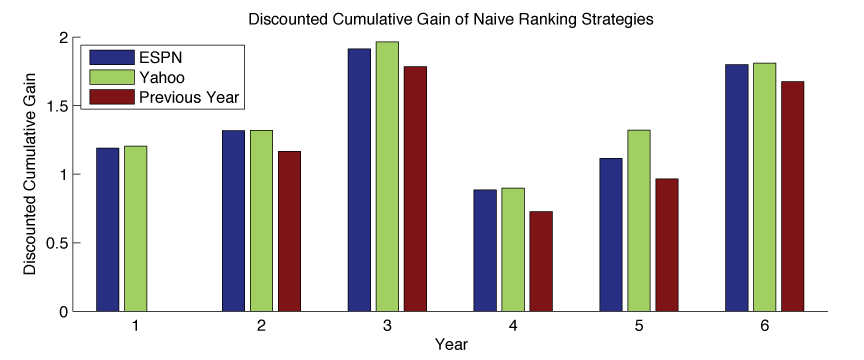
\includegraphics[width=5in]{media/dcg_naive.png}
\caption{: DCG of ESPN / Yahoo preseason rankings over the years, along with a na�ve method of using the previous year�s final rankings as the next year�s preseason rankings.}
\end{centering}
\end{figure}

%#####################################################################################
%	Models and Methods
%#####################################################################################

\section{Models and Methods}



\subsection{Regression}



%#####################################################################################
%	Results
%#####################################################################################

\section{Results}

%#####################################################################################
%	Conclusions
%#####################################################################################

\section{Conclusions}

%#####################################################################################
%	Bibliography
%#####################################################################################

\newpage

\section{Bibliography}

\end{document}


